\begin{enumerate}
	\item \textbf{Stampa resoconto guadagno.}\\
	      \begin{tabularx}{\textwidth}{|X|X|}
			  \hline
			  \vspace{.01mm}
		      SELECT
		      SUM(Ordini.PrezzoTotale)
		      FROM
		      Ordini
		      WHERE
		      Ordini.Data <= CURRENT\_TIMESTAMP
		      AND Ordini.Data >= DATE\_ADD(CURRENT\_TIMESTAMP, INTERVAL -7 DAY);
			   &
			   \raisebox{-\totalheight}{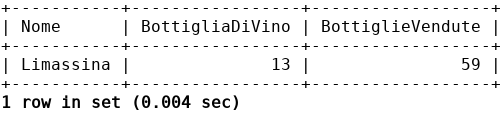
\includegraphics[width=0.47\textwidth, keepaspectratio]{src/queryIndici/assets/Query1.png}}
		      \\
		      \hline
	      \end{tabularx}
	\item \textbf{Bottiglia/e di vino più venduta/e dell'anno 2019 con la relativa quantità.}\\
	      \begin{tabularx}{\textwidth}{|X|X|}
		      \hline
			  \vspace{.01mm}
		      CREATE VIEW OrdineQuantita AS
		      SELECT
		      Vini.Nome,
		      SUM(Dettagli.QuantitaBottiglie) AS BottiglieVendute
		      FROM Dettagli,
		      BottiglieDiVino,
		      Vini, Ordini
		      WHERE
		      Dettagli.BottigliaDiVino = BottiglieDiVino.Id
		      AND Vini.Nome = BottiglieDiVino.Vino AND DATE\_FORMAT(Ordini.Data, '\%Y') = '2019'
		      AND Ordini.Id = Dettagli.Ordine
		      GROUP BY
		      Dettagli.BottigliaDiVino;
		      \newline\newline
		      SELECT
		      OrdineQuantita.Nome,
		      OrdineQuantita.BottiglieVendute
		      FROM
		      OrdineQuantita
		      WHERE
		      OrdineQuantita.BottiglieVendute IN (
		      SELECT
		      MAX(OrdineQuantita.BottiglieVendute)
		      FROM
		      OrdineQuantita
		      );
			   &
			   \raisebox{-\totalheight}{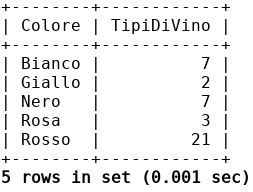
\includegraphics[width=0.47\textwidth , keepaspectratio]{src/queryIndici/assets/Query2.png}}
		      \\
		      \hline
		  \end{tabularx}
		  \vspace{1cm}
	\item \textbf{Lista dei vini prodotti con la relativa tipologia di uva utilizzata e il fornitore di quest'ultima.}\\
	      \begin{tabularx}{\textwidth}{|X|X|}
		      \hline
			  \vspace{.01mm}
		      SELECT DISTINCT
		      Vini.Nome AS Vino,
		      Uva.TipoUva as TipoUva,
		      Informazioni.Nome as Fornitore
		      FROM
		      Vini,
		      Uva,
		      Informazioni,
		      Aziende
		      WHERE
		      Vini.Uva = Uva.Id
		      AND Uva.Fornitore = Aziende.PartitaIVA
		      AND Aziende.InformazioniAggiuntive = Informazioni.Id;
			   &
			   \raisebox{-\totalheight}{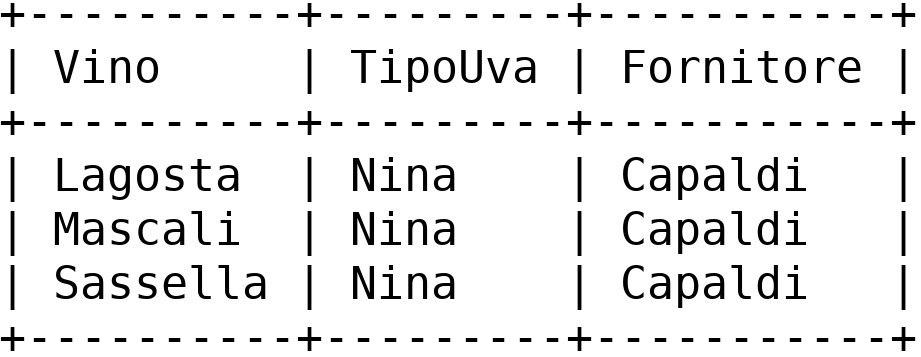
\includegraphics[width=0.47\textwidth , keepaspectratio]{src/queryIndici/assets/Query3.png}}
			   \\
		      \hline
	      \end{tabularx}
	\item \textbf{Lista dei dipendenti (ordinati in ordine alfabetico) che sono supervisori di altri dipendenti.}\\
	      \begin{tabularx}{\textwidth}{|X|X|}
		      \hline
			  \vspace{.01mm}
		      SELECT
		      DISTINCT D1.Cognome,
		      D1.Nome
		      FROM
		      Dipendenti as D1,
		      Dipendenti as D2
		      WHERE
		      D2.Referente = D1.CodiceFiscale
		      ORDER BY
		      D1.Cognome,
		      D1.Nome;
			   &
			   \hspace{1.8cm}
			   \raisebox{-\totalheight}{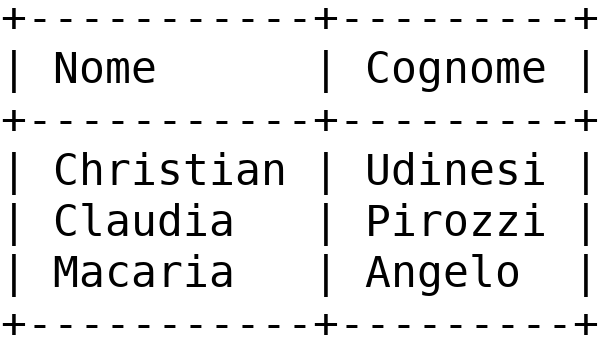
\includegraphics[width=0.3\textwidth]{src/queryIndici/assets/Query4Limited.png}}
		      \\
		      \hline
	      \end{tabularx}
	\item \textbf{Lista dei dipendenti (nome, cognome) che hanno lavorato il giorno 22 ottobre 2019, con inizio e fine turno, ordinati in modo decrescente in base all'inizio del turno.}\\
	      \begin{tabularx}{\textwidth}{|X|X|}
		      \hline
			  \vspace{.01mm}
		      SELECT
		      D.Nome,
		      D.cognome,
		      T.InizioTurno,
		      T.FineTurno
		      FROM
		      Dipendenti as D,
		      Turni as T
		      WHERE
		      T.Dipendente = D.CodiceFiscale
		      AND DATE\_FORMAT(T.InizioTurno, '\%Y-\%m-\%d') = '2019-10-22'
		      ORDER BY
		      T.InizioTurno DESC;
			   &
			   \raisebox{-\totalheight}{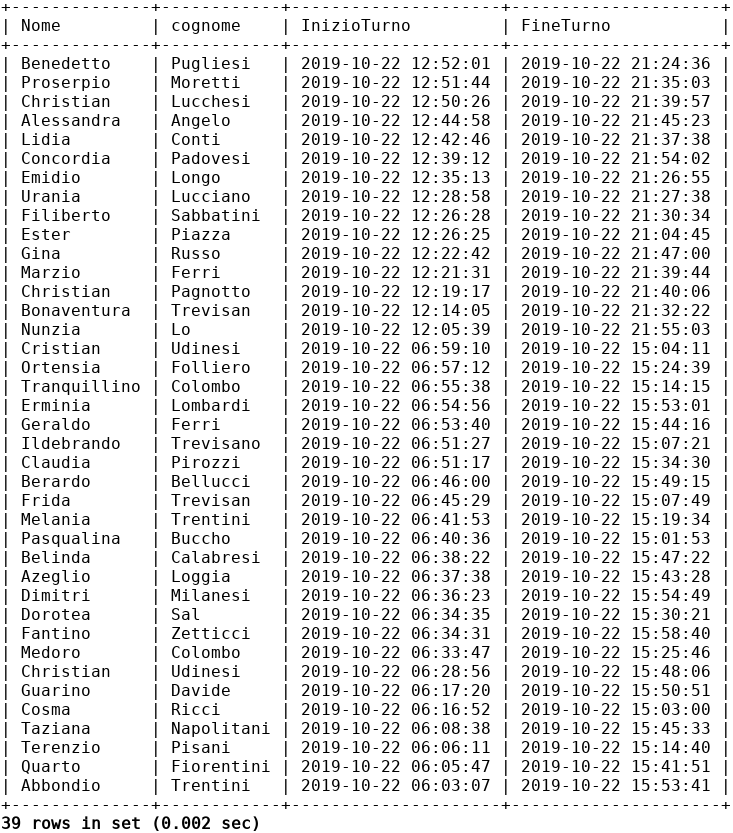
\includegraphics[width=0.47\textwidth]{src/queryIndici/assets/Query5.png}}
		      \\
		      \hline
	      \end{tabularx}
	\item \textbf{Lista degli acquirenti che hanno acquistato il maggior valore di bottiglie di vino dalla cantina.}\\
	      \begin{tabularx}{\textwidth}{|X|X|}
		      \hline
			  \vspace{.01mm}
		      CREATE VIEW SpeseTotali AS
		      SELECT
		      Ordini.Acquirente,
		      SUM(Ordini.PrezzoTotale) AS SpesaTotale
		      FROM
		      Ordini
		      GROUP BY
		      Ordini.Acquirente;
		      \newline\newline
		      SELECT
		      SpeseTotali.Acquirente,
		      SpeseTotali.SpesaTotale
		      FROM
		      SpeseTotali
		      WHERE
		      SpeseTotali.SpesaTotale IN (
		      SELECT
		      MAX(SpeseTotali.SpesaTotale)
		      FROM
		      SpeseTotali
		      );
			   &
			   \raisebox{-\totalheight}{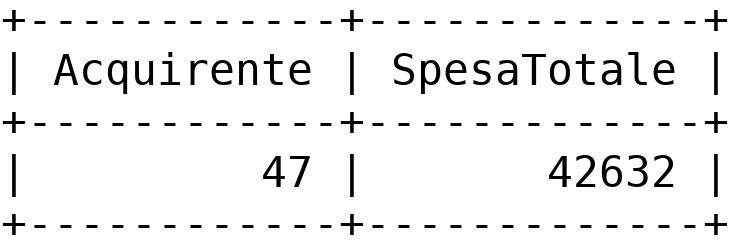
\includegraphics[width=0.47\textwidth]{src/queryIndici/assets/Query6.png}}
		      \\
		      \hline
	      \end{tabularx}
\end{enumerate}